\documentclass[dissertation.tex]{subfiles}
\begin{document}

\chapter{Exploration of learned representations}

\section{Token-level embeddings}

Filter to notes

\begin{figure}[htpb]
    \centering
    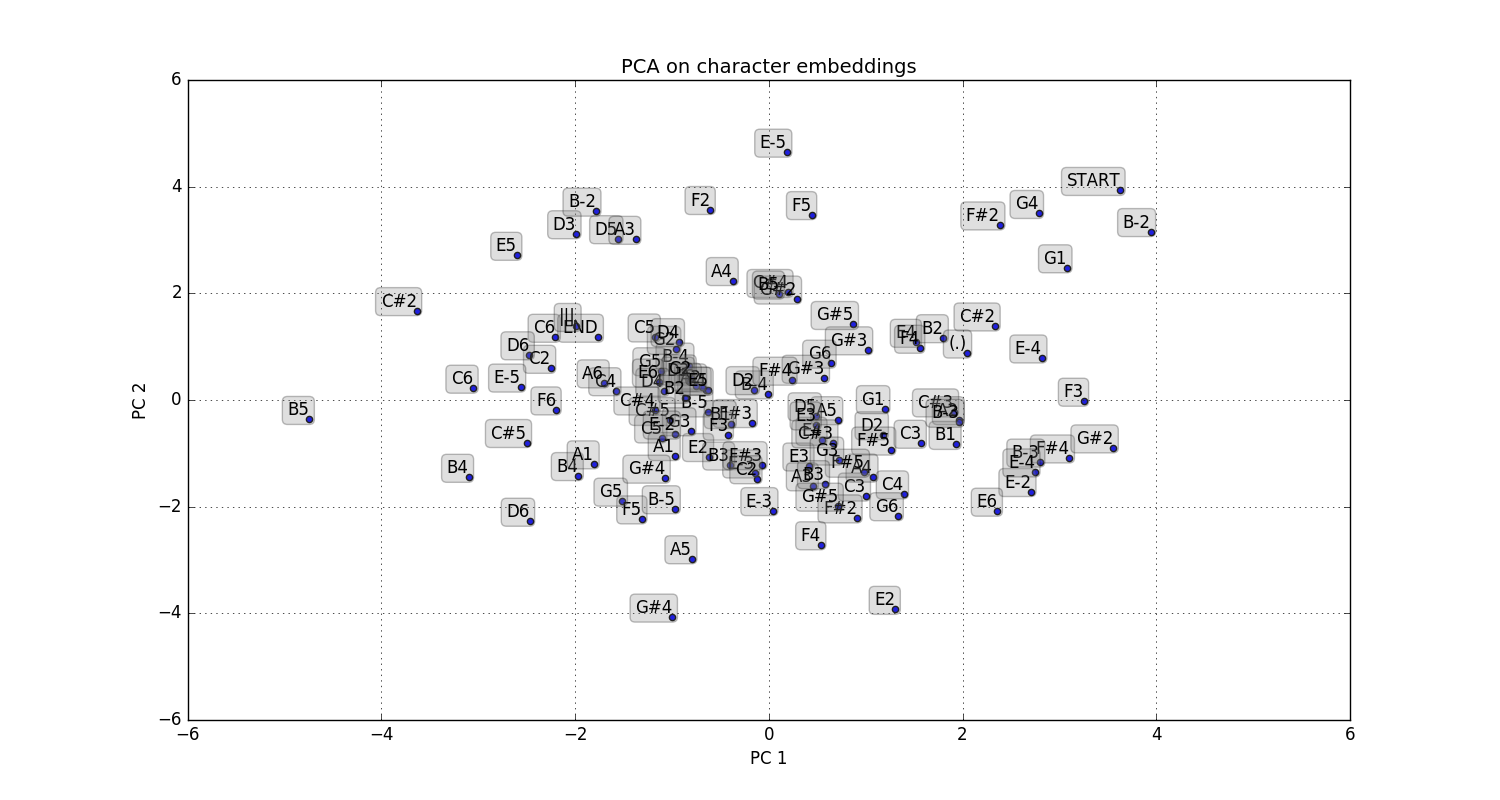
\includegraphics[width=0.8\linewidth]{Figures/PCA-notes.png}
    \caption{PCA embedding of note tokens}
    \label{fig:pca-notes}
\end{figure}

\begin{figure}[htpb]
    \centering
    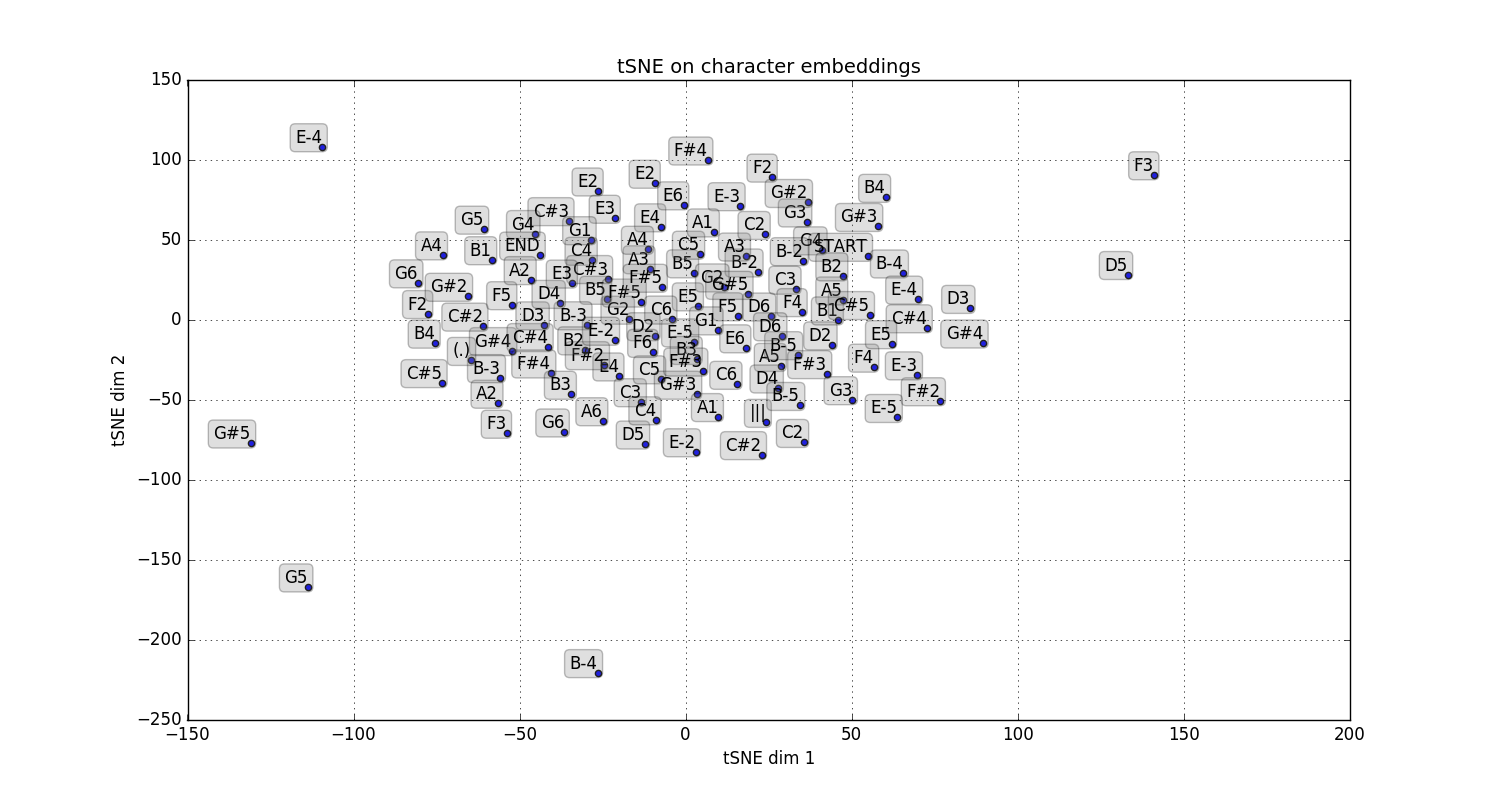
\includegraphics[width=0.8\linewidth]{Figures/tSNE-notes.png}
    \caption{tSNE embedding of note tokens}
    \label{fig:tsne-notes}
\end{figure}

\subsection{Variable-length embeddings}

\todo{LSTM hidden state after consuming chord (chord boundary, do they
    cluster?), phrase (up to fermata, do similar phrases embed similarly),
    whole pieces (difficult to evaluate)}

\section{LSTM Layer activations}

\todo{Probabilistic piano roll}

\subsection{Interesting neurons}


\printbibliography

\end{document}
